%%%%%%%%%%%%%%%%%%%%%%%%%%%%%%%%%%%%%%%%%
% Beamer Presentation
% LaTeX Template
% Version 1.0 (10/11/12)
%
% This template has been downloaded from:
% http://www.LaTeXTemplates.com
%
% License:
% CC BY-NC-SA 3.0 (http://creativecommons.org/licenses/by-nc-sa/3.0/)
%
%%%%%%%%%%%%%%%%%%%%%%%%%%%%%%%%%%%%%%%%%

%----------------------------------------------------------------------------------------
%	PACKAGES AND THEMES
%----------------------------------------------------------------------------------------

\documentclass{beamer} 
%\usepackage[font=small,skip=0pt]{caption}
%\setbeamertemplate{caption}[numbered]
%\captionsetup[figure]{font=small,skip=0pt}
\mode<presentation> {

% The Beamer class comes with a number of default slide themes
% which change the colors and layouts of slides. Below this is a list
% of all the themes, uncomment each in turn to see what they look like.

%\usetheme{default}
%\usetheme{AnnArbor}
%\usetheme{Antibes}
%\usetheme{Bergen}
%\usetheme{Berkeley}
%\usetheme{Berlin}
%\usetheme{Boadilla}
%\usetheme{CambridgeUS}
%\usetheme{Copenhagen}
%\usetheme{Darmstadt}
%\usetheme{Dresden}
%\usetheme{Frankfurt}
%\usetheme{Goettingen}
%\usetheme{Hannover}
%\usetheme{Ilmenau}
%\usetheme{JuanLesPins}
%\usetheme{Luebeck}
\usetheme{Madrid}
%\usetheme{Malmoe}
%\usetheme{Marburg}
%\usetheme{Montpellier}
%\usetheme{PaloAlto}
%\usetheme{Pittsburgh}
%\usetheme{Rochester}
%\usetheme{Singapore}
%\usetheme{Szeged}
%\usetheme{Warsaw}

% As well as themes, the Beamer class has a number of color themes
% for any slide theme. Uncomment each of these in turn to see how it
% changes the colors of your current slide theme.

%\usecolortheme{albatross}
%\usecolortheme{beaver}
%\usecolortheme{beetle}
%\usecolortheme{crane}
%\usecolortheme{dolphin}
%\usecolortheme{dove}
%\usecolortheme{fly}
%\usecolortheme{lily}
%\usecolortheme{orchid}
%\usecolortheme{rose}
%\usecolortheme{seagull}
%\usecolortheme{seahorse}
%\usecolortheme{whale}
%\usecolortheme{wolverine}

%\setbeamertemplate{footline} % To remove the footer line in all slides uncomment this line
%\setbeamertemplate{footline}[page number] % To replace the footer line in all slides with a simple slide count uncomment this line

%\setbeamertemplate{navigation symbols}{} % To remove the navigation symbols from the bottom of all slides uncomment this line
}
\graphicspath{{Figures/}}
\usepackage{graphicx} % Allows including images
\usepackage{booktabs} % Allows the use of \toprule, \midrule and \bottomrule in tables
\usepackage[ruled,boxed]{algorithm2e}
\newcommand{\HRule}{\rule{\linewidth}{0.5mm}} % New command to make the lines in the title page
%\newtheorem{lemma}{Lemma}
% \newtheorem{thm}{Theorem}
\newtheorem{thm}{{\break \noindent {\bf Theorem}}}

\newcommand{\loc}   	{ {\mathrm {Loc}} }
\newcommand{\ACONN}   { {\mathrm {A\mbox{-}CONN}} }
\newcommand{\SCONN}   { {\mathrm {S\mbox{-}CONN}} }
\newcommand{\ARCONN}   { {\mathrm {AR\mbox{-}CONN}} }
\newcommand{\SRCONN}   { {\mathrm {SR\mbox{-}CONN}} }
\newcommand{\GV}   { {\mathrm {G=(V,E_G,Loc,p)} }}

\newcommand{\fConn}   	{ {\mathrm {Conn}} }

\newcommand{\nReq}    { {n_{req}} }
\newcommand{\boldS}   { \mathbf{S}}
\newcommand{\DCH}     { {DCH} }

%% -- older paper --

\newcommand{\starEqual}   { {\;{\scriptstyle *} \! =} }
\newcommand{\plusEqual}   { {\;{\scriptstyle +} \! =} }
%\newcommand{\plusplus}    { {\scriptstyle \!+\!+} }

%\newcommand{\starEqual}   { {\; {\mathtt *=}} }
%\newcommand{\plusEqual}   { {\; \mathtt{+=}} }

% --------------------
\newcommand{\set}[1]    {{ \{ #1 \} }}
\newcommand{\iin}[1]    {\hspace*{#1in}}

\newcommand{\ol}[1]     {\overline{#1}}

\newcommand{\Prob}[1]   { {\bf \mathrm{Prob}} \left[ #1 \right] }
\newcommand{\aPr}	{ {\mathrm  {Pr}} }

\newcommand {\nwline} {\hfill\break}

%----------------------------------------------------------------------------------------
%	TITLE PAGE
%----------------------------------------------------------------------------------------

\title[Prob. Connectivity of USN]{Tree Bound on Probabilistic Connectivity of Underwater Sensor Networks} % The short title appears at the bottom of every slide, the full title is only on the title page

\author{Md Asadul Islam and Professor Ehab S. Elmallah} % Your name
\institute[UofA] % Your institution as it will appear on the bottom of every slide, may be shorthand to save space
{
University of Alberta \\ % Your institution for the title page
\medskip
\textit{\{mdasadul,elmallah\}@ualberta.ca} % Your email address
}
\date{\today} % Date, can be changed to a custom date

\begin{document}

\begin{frame}
\titlepage % Print the title page as the first slide
\end{frame}

\begin{frame}
\frametitle{Overview} % Table of contents slide, comment this block out to remove it
\tableofcontents % Throughout your presentation, if you choose to use \section{} and %\subsection{} commands, these will automatically be printed on this slide as an overview of your presentation
\end{frame}

%----------------------------------------------------------------------------------------
%	PRESENTATION SLIDES
%----------------------------------------------------------------------------------------
\section{Problem Formulation and Thesis Contributions}
%------------------------------------------------

%------------------------------------------------

\begin{frame}
\frametitle{Why UWSNs?}
UWSNs fuelled by many important underwater sensing applications and services such as

\begin{itemize}
\item Scientific applications
\item Industrial applications
\item Military and homeland security applications
\item Humanitarian applications
\end{itemize}
\end{frame}

%------------------------------------------------
\section{Challenges}
\begin{frame}

\frametitle{Challenges of the underwater communication}
\begin{block}{Radio Communication}
\begin{itemize}
\item suffer strong attenuation in salt water
\item short distances (6-20 m) and low data rates (1 Kbps)
\item require large antennas and high transmission power
\end{itemize}
\end{block}

\begin{block}{Optical Communication}
\begin{itemize}
\item strongly scattered and absorbed underwater
\item  limited to short distances (≤ 40 m)
\end{itemize}
\end{block}

\begin{block}{Acoustic Communication}
\begin{itemize}
\item suffers from attenuation, spreading, and noise 
\item very long delay because of low propagation speed.
\item it is most practical method upto now 
\end{itemize}
\end{block}
\end{frame}

%------------------------------------------------
\section{Node Deployment Strategy}
\begin{frame}
\frametitle{Node Deployment Strategy}
\begin{block}{Static Deployment}
\begin{itemize}
\item nodes attached to underwater ground, anchored buoys, or docks
\item are not subject to move
\end{itemize}
\end{block}
\begin{block}{Semi-mobile Deployment}
\begin{itemize}
\item nodes attached to a free floating buoy
\item subject to small scale movement 
\end{itemize}
\end{block}
\begin{block}{Mobile Deployment}
\begin{itemize}
\item composed of drifters with self/noself mobile capability
\item are subject to large scale movement
\item maintaining connectivity is important to perform localization, routing etc. 
\end{itemize}
\end{block}
\end{frame}
%------------------------------------------------

%------------------------------------------------
\begin{frame}
\frametitle{Node Locality Sets}
\begin{itemize}
\item  $V=V_{sense}\cup V_{relay}$ the set of nodes in a given UWSN
\item The geographic area considered rectangles of a superimposed grid layout.
%
\item At time $T,$ each node $x$ can be in any one of a possible
set of grid rectangles denoted $\loc(x)= \{ x[1], x[2], \ldots \}$.

\item Node $x$ can be grid rectangle $x[i]$ with a certain probability $p_x(i)$. 
\item Truncate some locality sets of low probability for convenience thus, $\sum_{x[i] \in \loc(x)} p_x(i) \leq 1$, if $\loc(x)$ is truncated.
\end{itemize}

\begin{figure}
\includegraphics[width=4 in, height=1 in]{LocalitySet.pdf}
\caption{Network with Probabilistic locality set}
\end{figure}
\end{frame}
%------------------------------------------------

%------------------------------------------------
\begin{frame}
\frametitle{Node Reachability}
\begin{itemize}
\item node $x$ can reach node $y$ if the acoustic signal strength from $x$ to $y$ (and vice versa) exceeds a certain threshold value.
\item we set $E_G(x[i],y[j])= 1$ iff the two nodes $x$ and $y$ can reach each other if they are located anywhere in their respective rectangles $x[i]$ and $y[j]$.

\item connectivity between $x$ and $y$ is ignored if 
they can reach each other at some (but not all) pairs of points in their respective rectangles.

\item ignoring connectivity in such cases results
in computing lower bounds on the network connectivity, as required.
\end{itemize}
\end{frame}
%------------------------------------------------

%\begin{frame}
%\frametitle{Kinematic Model}
%We note that this area is new to networking researchers where the obtained analytical
%results are rooted in the mathematically deep field of fluid dynamics.
%\begin{itemize}
%\item A particle pathline is a path followed by an individual particle in a flow
%\item A \textit{stream} function denoted  by $\psi$ measures the volume flow rate per unit depth.
%\item Curves where $\psi$ is constant are called \textit{streamlines}
%\end{itemize}
%The stream function can be presented \\
%\begin{equation}\label{eq:sf}
%\psi(x,y,t)=-\tanh{[\frac{y-B(t)\sin(k(x-ct))}{\sqrt{1 + k^2 B^2(t) \cos^2(k(x-ct))}} ]} + cy
%\end{equation}
% where $  B(t) = A + \epsilon \cos(\omega t)$  and the x and y velocities are given by
% 
% \begin{equation}\label{eq:lf}
%\dot{x}=-\frac{\partial \psi}{\partial y} ; \dot{y}=\frac{\partial \psi}{\partial x}
%\end{equation}
%\end{frame}
%%------------------------------------------------
%\begin{frame}
%\frametitle{Kinematic Model (cont.)}
%\vspace{-1em}
%\begin{figure}[!htb]
%\begin{minipage}[]{0.5\linewidth}
%\includegraphics[width=2 in, height=1.5 in]{3D1.pdf}
%\vspace{-1em}
% \caption{ A 3D plot of \ref{eq:sf}}
% \label{fig:kme3d}
% \end{minipage}
% \begin{minipage}{0.45\linewidth}
% 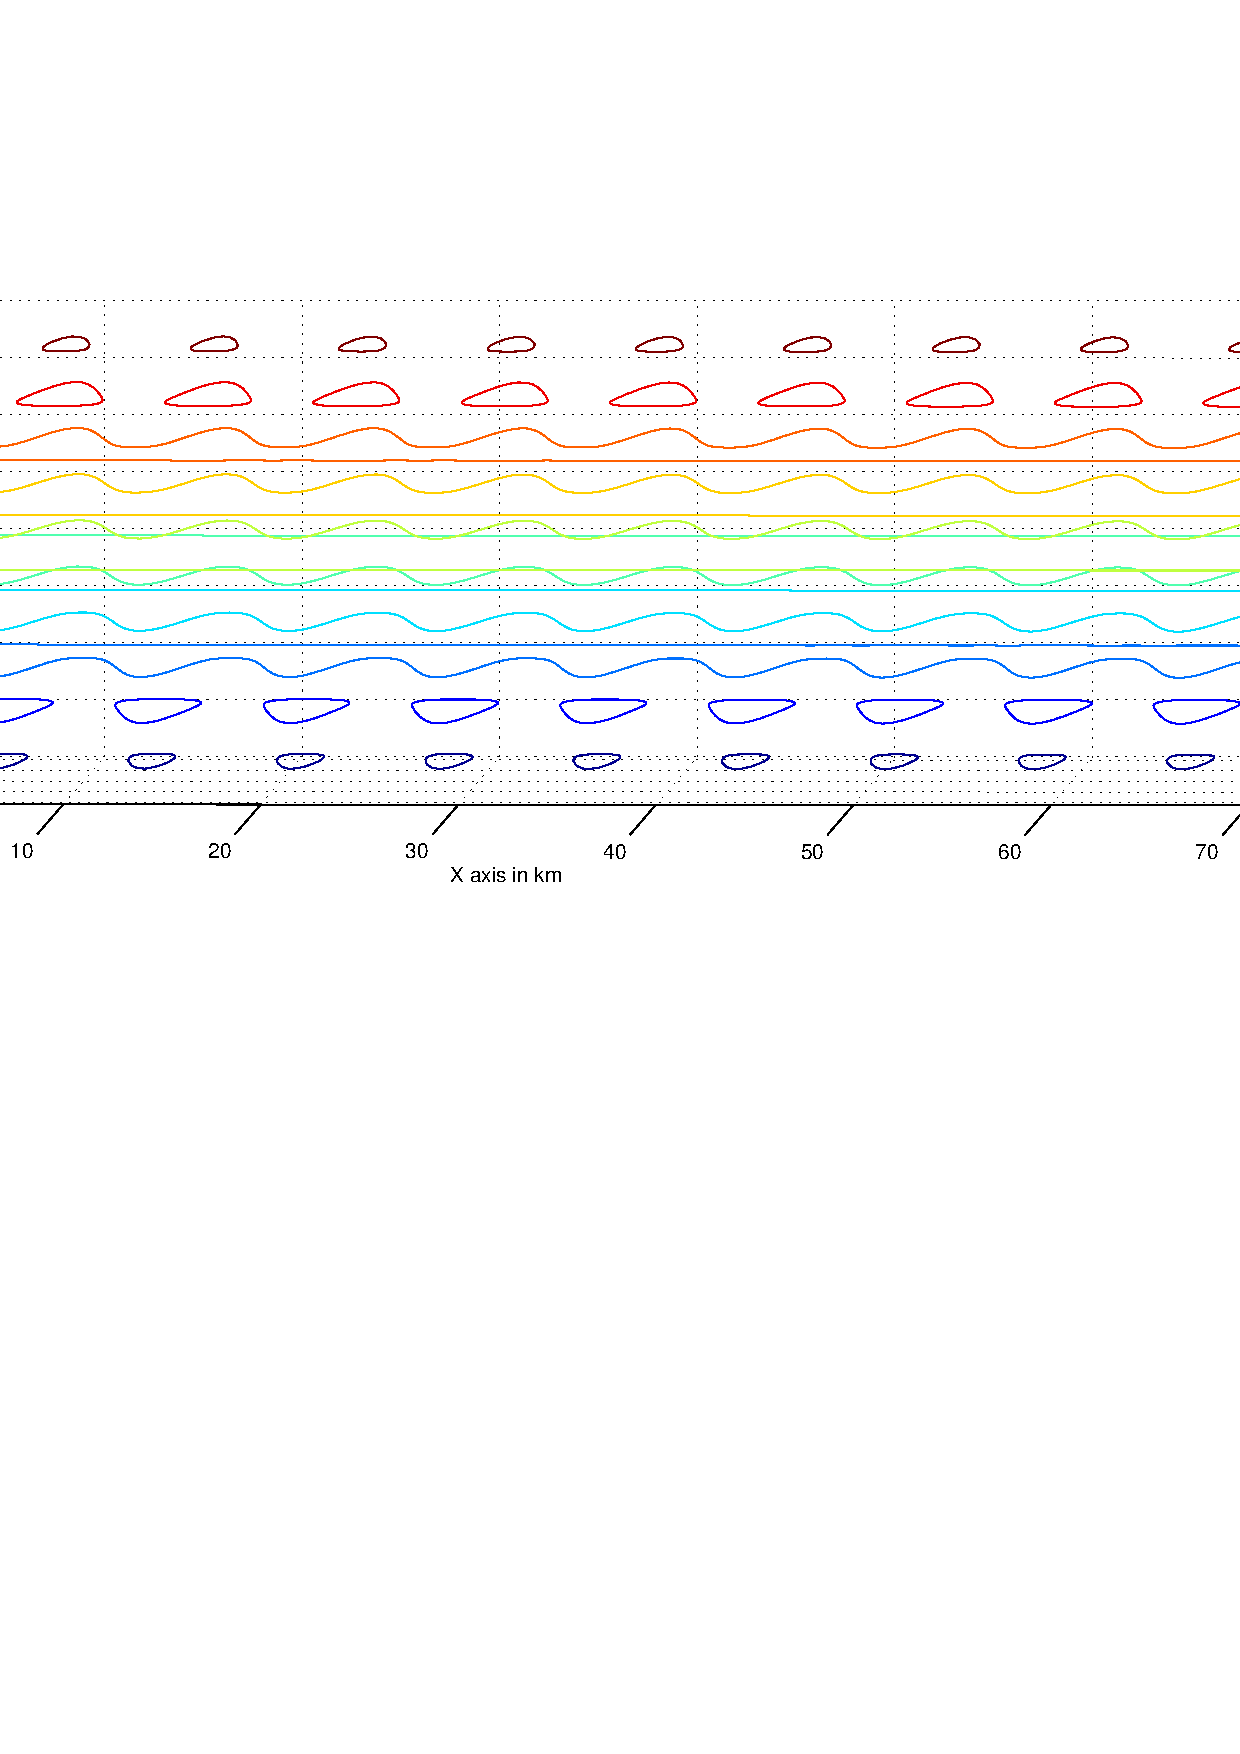
\includegraphics[width=2 in, height=1.5 in]{MCM.pdf}
% \vspace{-1em}
% \caption{ A plot of  \ref{eq:sf} at $t=0$.}
% \label{fig:kme}
% \end{minipage}
%\end{figure}
%\vspace{-1em}
%\begin{figure}[!htb]
%\begin{minipage}[]{.5\linewidth}
%\includegraphics[width=2 in, height=1 in]{start_end_50.pdf}
%\vspace{-1em}
% \caption{ Start and end points of 50 nodes}
%\label{fig:res11}
%\end{minipage}
%\begin{minipage}{.45\linewidth}
%\includegraphics[width=1 in, height=1 in,angle=-90]{points1.pdf}
%\vspace{-0.5em}
% \caption{probabilistic distribution}
%\label{fig:ges11}
% \end{minipage}
%\end{figure}
%\end{frame}
%------------------------------------------------
\section{Problem Definition}
\begin{frame}
\frametitle{Problem Definition}
We define four probabilistic connectivity problem. They are 
\begin{itemize}
\item $\ACONN$ problem
\item $\SCONN$ problem

\end{itemize}
\end{frame}
%-----------------------------------------------
%-----------------------------------------------
\begin{frame}
\frametitle{the $\ACONN$  and $\SCONN$ problems}
\begin{definition}[\textbf{the $A$-$CONN$ problem}]
\normalfont
Given a probabilistic network $G$ with no relay nodes, compute the probability $Conn(G)$ that the network is in a state where the sink node $s$ can reach all sensor nodes. 
\end{definition}

\begin{definition}[\textbf{the $S$-$CONN$ problem}]
Given a probabilistic network $G$ with no relay nodes, and a required number of sensor nodes $n_{req}\leq |V_{sense}|$, compute the probability $Conn(G,n_{req})$ that the network is in a state where the sink node $s$ can reach a subset of sensor nodes having at least $n_{req}$ sensor nodes. 
\end{definition}


\end{frame}

%-----------------------------------------------

%-----------------------------------------------

\begin{frame}
\frametitle{Network State}
\begin{itemize}
\item A probabilistic graphs arises when network is in some particular network states.
\item A state $S$ of $V$ can be specified by $\{v_1[i_1], v_2[i_2], . . . , v_n[i_n]\}$
\item If locations are independent, we have $Pr(S) =\prod_{v_{\alpha}\in V} p_{v_\alpha[i_\alpha]}$.

\item In the $A$-$CONN$ problem, a state is \textbf{operating} if the
sink $s$ can reach all sensor nodes in $V_{sense}$ . 
\item Similarly, in the $S$-$CONN$ problem, a state $S$ is \textbf{operating} if the sink node $s$ can reach a $n_{req}$ sensor
nodes.
\end{itemize}
\vspace*{-0.5 cm}
\begin{columns}
\vspace*{-0.5 cm}

\column{0.8\linewidth}
\begin{figure}[h]
\centering
\includegraphics[width=1.8 in, height=1 in]{Figure1.pdf}
\vspace*{-0.5 cm}
 \caption{ An example network}
\end{figure}
\end{columns}
\end{frame}
%------------------------------------------------
%\subsection{Thesis Contribution}
%------------------------------------------------
\section{Overview on $k$-Trees and Partial $k$-Trees}
%------------------------------------------------

\begin{frame}
\frametitle{$k$-Trees and Partial $k$-Trees}
\vspace{-0.7em}
\begin{definition} For a given integer $k\geq 1$, the class of $k$-trees is defined as follows
\begin{enumerate}
\item A $k$-clique is a $k$-tree.
\item If $G_n$ is a $k$-tree on $n$ nodes then the graph $G_{n+1}$ obtained by adding a new node adjacent to every node in $k$-clique of $G_n$. 
\end{enumerate}
\end{definition}
\vspace{-1em}
\begin{figure}[!htb]
\begin{minipage}[]{0.4\linewidth}
\includegraphics[width=1 in, height=.8 in]{Ch3f2.pdf}
\vspace{-1em}
 \caption{a fragment of a 3-tree}
 \label{fig:f3t1}
 \end{minipage}
 \begin{minipage}{0.45\linewidth}
 \includegraphics[width=1 in, height=0.8 in]{Ch2f2.pdf}
  \vspace{-1em}
 \caption{a fragment of partial 3-tree}
 \label{fig:f3t2}
 \end{minipage}
\end{figure}
\vspace{-1em}
A partial $k$-tree is a $k$-tree possibly missing some edges
and a \textit{$k$-perfect elimination sequence} $(k\mbox{-}PES)$ of  $G$ is an ordering $(v_1,v_2,\ldots,v_r)$ of $v(G)$
\vspace{-0.5em}
\begin{example}
\normalfont 
For the graph $G$ in figure , $(v_a,v_b,v_i,v_j,v_k,v_l)$ is a 3-$PES$. 
\end{example}
\end{frame}
%%------------------------------------------------
%%\subsection{Graphs with Bounded Tree-width}
%%-----------------------------------------------
%------------------------------------------------
%\subsection{Dynamic Programing on Partial $k$-Trees}
\section{Probabilistic Connectivity of Tree Network}
%\subsection{Notation and Definition}
%\subsection{Pseudo-code for $\SRCONN$ problem on tree network}
%\subsection{Running time Analysis}
\begin{frame}
\frametitle{Probabilistic Connectivity of Tree Network}
\begin{itemize}
\item Notation and Definition
\item Pseudo-code for $\SCONN$ problem on tree network
\item Running time Analysis
\end{itemize}
\end{frame}
\begin{frame}
\frametitle{Notation and definition}
\begin{columns}[t]
\column{0.65\textwidth}
\vspace{-1.7em}
\begin{itemize}
\item	$type(x)$: $type(x)= 0$ and 1 if $x$ is a relay node and 
 a sensor node respectively.

\item	$n_{sense}(X)$: \# of sensor nodes in a given subset  of nodes $X\subseteq V$.

\item   $n_{relay}(X)$: \# of relay nodes in a given subset of nodes $X\subseteq V$.

\item $n(X)=n_{sense} + n_{relay}$.

\item $n_{sense,min}(X)$: The minimum number of sensor nodes in a given subset $X\subseteq V$. So,\\
\centerline{
$n_{sense,min}(X)=max(0,n_{req}-n_{sense}(\overline{X}))$
}
\end{itemize}
\column{0.35\textwidth}
\begin{figure}[!htb]
\centering
\includegraphics[width=1.7 in, height=0.8 in]{Ch4f1.pdf}
 \caption{ A tree network}
\label{fig:es31}
\end{figure}
\end{columns}

\begin{example}
\normalfont
In figure , consider node $x_2$. $n(V_{x_2})=8$ where $n_{sense}(V_{x_2})=5$ and $n_{relay}(V_{x_2})=3$. Assuming $n_{req}=5$ in an instance of the $\SCONN$ problem then $n_{sense,min}(V_{x_2})=3=n_{req}-n_{sense}(\{s,x_1\})=5-2$. 
\end{example}
\end{frame}
%------------------------
\begin{frame}
\frametitle{$\SRCONN$ problem}
\begin{figure}
\includegraphics[scale=1]{Tree.pdf}
\caption{Table merge in Tree networks and $n_{req}=5$}
\end{figure}
\end{frame}

\begin{frame}
\frametitle{Pseudo-code for function Conn}
\vspace{-1.7em}
   % --------------- Function E2P ---------------
    \begin{figure}[htbp]
    % \begin{figure}[!ht]
    \small
\begin{center}
%\fbox{
    \begin{minipage}[t]{5 in}
    \renewcommand{\baselinestretch}{1}
    %
    {\bf Function $\fConn (G, T, \nReq)$}\\
	{\bf Input:}
	\begin{minipage}[t]{5in}
	the $SR$-$CONN$ problem where $G$ has a tree
	topology $T$ with no relay leaves
	\end{minipage}
	{\bf Output:}
	\begin{minipage}[t]{5in}
	$Conn(G, \nReq)$
	\end{minipage}
%
%\nwline
%	{\bf Notation:}
%	\begin{minipage}[t]{2.75in}
%	\end{minipage}
% --------------------
% initialization
   1.  \begin{minipage}[t]{5in}
       {\bf foreach} (node $x$ and a valid location index $i$) \\
         \iin{0.20} set $R_x(i, type(x) )= 1$ 
       \end{minipage}       
   2.  \begin{minipage}[t]{5in}
       {\bf while} ($T$ has at least 2 nodes) \\
       \{
       \end{minipage}
       \\
   3.  \iin{0.20} \begin{minipage}[t]{5 in}
   		  Let $y$ be a non-sink leaf of $T$, and $x= parent(y)$
		  \end{minipage}
		  \\
   4.  \iin{0.20} \begin{minipage}[t]{5 in}
   		  {\bf foreach} (key $(i,count) \in R_y$)
		       $R_y (i,count) \starEqual p_y(i)$
		  \end{minipage}
		  \\
   5.  \iin{0.20} \begin{minipage}[t]{5in}
   		  set $R'_x= \phi$
		  \end{minipage}
		  \\
   6.  \iin{0.20} \begin{minipage}[t]{5in}
   		  {\bf foreach} (pair of keys
		       		$\begin{array}[t]{l}
				 (i_x, count_x) \in R_x \mbox { and }
		   		 (i_y, count_y) \in R_y)
				 \end{array}
				$ \\ 
		  \{
		  \end{minipage}
		  \\
   7.  \iin{0.40} \begin{minipage}[t]{5 in}
   		  $count= \min (\nReq, count_x + count_y)$
		  \end{minipage}
		  \\
%   8.  \iin{0.40} \begin{minipage}[t]{5 in}
%   		  $count_{x,min}= \begin{array}[t]{l}
%		  		  type(x) + n_{y,min} + 
%		       	   	  \sum_{z \in \DCH(x)} n_{z,min}
%				  \end{array}$
%		  \end{minipage}
%		  \\
  8.  \iin{0.40} \begin{minipage}[t]{5 in}
   		  {\bf if} ($count < n_{sense,min}(\{x\}\cup V_y \cup_{z\in DCH(x)} V_z)$) {\bf continue} 
		  \end{minipage}
		  \\
   9.  \iin{0.35} \begin{minipage}[t]{5in}
   		  $R'_x (i_x,count) \plusEqual$ 
		  	$\begin{array}[t]{l}
			 R_y(i_y,count_y) \times 
			 R_x(i_x,count_x) \times 
			 E_G(x[i_x], y[i_y])
		  	 \end{array}$
		  \end{minipage}
		  \\
       \iin{0.40} \} \\
   10. \iin{0.20} \begin{minipage}[t]{5 in}
       		  set $R_x= R'_x$; remove $y$ from $T$
		   \end{minipage}
		   \\
       \iin{0.15} \} \\
   11. \begin{minipage}[t]{6 in}
       return $\sum_{s[i] \in \loc(s)} R_s(i,\nReq) * p_s(i)$
       \end{minipage}
       \\
    \end{minipage}	
%}
\end{center}
    \normalsize
    %
    \caption{Pseudo-code for function $\fConn$}
    \label{alg:Conn}
\vspace*{-0.1in}
    \end{figure}

\end{frame}
%-----------------------------------------
\begin{frame}
\frametitle{Running time}
Let $n$ be the number of nodes in $G$, and $\ell_{max}$ be the maximum
number of locations in the locality set of any node.

% ----------
\begin{theorem}
\normalfont
    Function $\fConn$ solves the $\SRCONN$ problem in
    $O(n \cdot n_{req}^2  \cdot \ell_{max}^2)$ time
\end{theorem}
{\bf Proof.}
We note the following.
\begin{itemize}
\item   Step 1: storing the tree $T$ require $O(n)$ time.

\item	Step 2: the main loop performs $n-1$ iterations.
	Each of Steps 3, 5, and 10 can be done in constant time.

\item	Step 4: this loop requires $O(\nReq \cdot \ell_{max})$ time.

\item	Step 6: this loop requires $O(n_{req}^2 \cdot \ell_{max}^2)$ iterations.
	Steps 7, 8, and 9 can be done in constant time.
\end{itemize}
Thus, the overall running time is $O(n \cdot n_{req}^2  \cdot \ell_{max}^2)$ time.

\begin{theorem}
\normalfont
    Function $\fConn$ solves the $\ARCONN$ problem in
    $O(n \cdot \ell_{max}^2)$ time

    % Overall: $O(n \cdot \ell_{max} + n \cdot \ell_{max}^2)$
\end{theorem}
\end{frame}
%-----------------------------------------

%------------------

\begin{frame}
\frametitle{Simulation Results for $\ACONN$ problem}

\begin{itemize}
\item Test Networks
\item Running Time
\item Connectivity for different partial $k$-trees
\item Effect of subgraph selection method
\end{itemize}
\end{frame}
%-----------------------------------------
\begin{frame}
\frametitle{Test Networks}
\vspace{-0.5em}
\begin{figure}[!htb]
\begin{minipage}{.8\linewidth}
\includegraphics[width=4 in, height=1.2 in]{NetworkI_paper.pdf}
\caption{Network $G_{10}$}
\label{fig:netI1}
\end{minipage}
\begin{minipage}{.8\linewidth}
\includegraphics[width=4 in, height=1.2 in]{NetworkI_paper_Relay.pdf}
\vspace{-0.7 cm}
\caption{Network $G_{10,3}$}
\label{fig:netIR}
\end{minipage}
\end{figure}

\end{frame}
%-----------------------------------------
%-----------------------------------------

%-----------------------------------------

%-----------------------------------------
\begin{frame}
\frametitle{Connectivity for different partial $k$-trees}
\begin{table}[!htb] 
      \centering
     \begin{tabular}{|c|c|c|c|}
     \hline
      k& Network $G_{10}$ & Network $G_{12}$ & Network $G_{15}$ \\
     \hline
      1 & 0.62&0.336& 0.82 \\\hline
2 &0.71 & 0.36& 0.99\\\hline
3 &0.75& 0.37& 1\\\hline
\end{tabular}
 \caption{Connectivity lower bounds using different partial $k$-trees}
 \label{Tab:acc}
\end{table}
\end{frame}
%-----------------------------------------
%-----------------------------------------


%-----------------------------------------
\begin{frame}
\frametitle{Running Time}
\begin{table}[!htb]
    %\caption{Global caption}
    \begin{minipage}{1\linewidth}
   
      \centering
     \begin{tabular}{|c|c|c|}
     \hline
         k& Network $G_{10}$ &Network $G_{10,3}$\\
     \hline
     1&90& 110 \\\hline
     2&1000 &6000	\\\hline
3 &6000&8000	 \\\hline
\end{tabular}
 \caption{Running time in milliseconds}
\label{Tab:rtym1}
    \end{minipage}
\end{table}

\end{frame}
%-----------------------------------------

%-----------------------------------------
\begin{frame}
\frametitle{Effect of adding relay nodes}

\begin{table}[!htb]
  \centering
 \begin{minipage}{.5\linewidth}
     \begin{tabular}{|c|c|c|}
     \hline
     k & Network $G_{10}$ & Network $G_{10,3}$  \\
     \hline
      1 & 0.30 & 0.86 \\\hline
	  2 & 0.54 & 0.96\\\hline
	  3 &0.60 & 0.98 \\\hline
\end{tabular}
    \end{minipage}
     \caption{Connectivity with respect to $k$}
      \label{Tab:SRC}   
\end{table}
\end{frame}
%-----------------------------------------

%-----------------------------------------
\begin{frame}
\frametitle{Effect of adding relay nodes for various node $R_{tr}$:}
\begin{itemize}
\item Each obtained curve exhibits a notable monotonic increasing behaviour as $R_{tr}$ increases. 
\item This behaviour is due to the appearance of more edges, and the potential increase in the probability of each edge as $R_{tr}$ increases. 
\item Increasing $R_{tr}$, however, requires increasing node energy consumption.
\item  To achieve a desired $Conn(G)$ value, a designer may utilize the obtained curves to assess the merit of increasing $R_{tr}$ versus deploying more relay nodes.
\end{itemize}
\begin{figure}[!htb]
\begin{minipage}{.9\linewidth}
\end{minipage}
\includegraphics[width=4 in, height=1.35 in]{NetworkI_woR-eps-converted-to.pdf}
\caption{Connectivity versus transmission range}
\label{Fig:NWOR}
\end{figure}

\end{frame}
%--------------

\begin{frame}
\frametitle{Concluding Remarks}
\begin{itemize}
\item This thesis is motivated by recent interest in UWSNs as a platform for preforming many useful tasks. 
\item A challenge arises since sensor nodes incur small scale and large scale movements that can disrupt network connectivity.
\item  Thus, tools for quantifying the likelihood that a network remains completely or partially connected become of interest.

\item the thesis has formalized 4 probabilistic connectivity problems, denoted $\ACONN,$ $ \SCONN, \ARCONN, \mbox{ and } \SRCONN$. 
\item The obtained results show that all of the 4 problems admit polynomial time algorithms on $k$-trees (and their subgraph), for any fixed $k$.
\end{itemize}
\end{frame}
%-----------------------------------------
\section{Future Research Directions}
%-----------------------------------------
\begin{frame}
\frametitle{Future Research Directions}
\begin{itemize}
\item Investigating the applicability of our algorithm to some other classes of graph to be a worthwhile direction.

\item It is interesting to analyze the delays incurred in typical data collection rounds.
\item It is worthwhile to investigate area coverage assuming a probabilistic locality model of the nodes.
\end{itemize}

\end{frame}
%-----------------------------------------


%-----------------------------------------
\begin{frame}
\frametitle{}
\begin{center}
\Huge Thanks!
\end{center}

\end{frame}
%-----------------------------------------
\end{document} 